\documentclass[11pt]{article}
\usepackage{amsmath, amssymb, amscd, amsthm, amsfonts}
\usepackage{graphicx}
\usepackage{hyperref}
\usepackage{tikz}

% Korean packages
\usepackage[T1]{fontenc}
\usepackage{CJKutf8}

\oddsidemargin 0pt
\evensidemargin 0pt
\marginparwidth 40pt
\marginparsep 10pt
\topmargin -20pt
\headsep 10pt
\textheight 8.7in
\textwidth 6.65in
\linespread{1.2}

\title{Winning the game Rummikub using () algorithm \\
	\large MATH 818.01 Midterm Survey
}
\author{Jiyoon Jeong}
\date{}

\newtheorem{theorem}{Theorem}
\newtheorem{lemma}[theorem]{Lemma}
\newtheorem{conjecture}[theorem]{Conjecture}

\newcommand{\rr}{\mathbb{R}}

\newcommand{\al}{\alpha}
\DeclareMathOperator{\conv}{conv}
\DeclareMathOperator{\aff}{aff}

\begin{document}
	
	\maketitle
	
	\begin{abstract}
		This survey presents an overview of the artificial intelligence that aims to win the board game, Rummikub. 
		We discuss the topological, linear-algebraic, and combinatorial aspects of Tverberg's theorem and its applications.  The survey contains several open problems and conjectures.
		
		
		
	\end{abstract}
	
	\section{Introduction}\label{section-introduction}
	
	\begin{CJK}{UTF8}{mj}
		한글 
	\end{CJK}
	
	Rummikub is a number-based board game. The players do not know the tiles that other players have and strategies that they choose to play; that is, every player lacks information during the game. Since there are 106 tiles and each player has only 14 tiles each initially, the player does not know which player has what tiles and what tiles are left untacted. In addition, it is not necessarily to give away every possible sets on the board, so it is comparatively hard to predict other players' strategies or status. For example, a player A has only finished one's initial meld, but do not give away sets anymore and has 23 tiles in this turn. The player B may have no sets to put down or perhaps trying to complete sets personally to finish the game in one final turn. Therefore, devising a program that aims to win the game Rummikub is likely to require some special algorithm or approach. Before getting into that, this paper will cover Case Studies of solving difficult games by using artificial intelligence (AI). Furthermore, the prior research of winning the game Rummikub in the way other than using AI will be covered as well.
	
	
	%Tverberg's theorem has been a cornerstone of combinatorial convexity for over fifty years. Its impact and influence is only comparable to that of the famous and classic theorems of Carath\'eodory and Helly. This gem lies at the crossroads of combinatorics, topology, and linear algebra, and continues to yield challenging and interesting open problems.  Its states the following.
	% If we denote by $\conv(S)$ the convex hull of a set $S \subset \rr^d$, it says the following
	
%	\begin{theorem}[Helge Tverberg 1966 \cite{Tverberg:1966tb}]
%		Given $(r-1)(d+1)+1$ points in $\rr^d$, there is a partition of them into $r$ parts whose convex hulls intersect.
%	\end{theorem}
%	
%	\begin{figure}
%		\centerline{
\includegraphics[scale=1]{fig1-Tverberg}}
%		\caption{An example of a Tverberg partition.  The partition is not unique.}
%	\end{figure}
%	
	%More formally, given $X\subset \rr^d$ of $(r-1)(d+1)+1$ points, there is a partition $X=X_1\cup \dots \cup X_r$ such that $\bigcap_{j=1}^r \conv X_j \ne \emptyset$. Such a partition is called a
	%\textit{Tverberg partition}. The number of points in this result is optimal, as a dimension-counting argument shows. In fact, if $X$ is in general enough position and in the partition $X=X_1\cup \ldots \cup X_r$ we have $1\le |X_j|\le d+1$ for every $j$, then $\bigcap_{j=1}^r \aff X_j$ is a single point if $|X|= (r-1)(d+1)+1$, and is empty if $|X|\le (r-1)(d+1)$.
	
	
	%The last decade has seen an impressive sequence of results around Tverberg's theorem.  The purpose of this survey is to give a broad overview of  the current state of the field and point out key open problems.  Other surveys covering different aspects of Tverberg's theorem can be found in \cite{Eckhoff:1979bi, Eck93survey, Matousek:2002td, BBZ17survey, de2017discrete, BZ17}.
	
	%The paper is organized as follows.  In sections \ref{section-information} and \ref{section-alphago} we describe the topological and colorful versions of Tverberg's theorem, which have received the most attention in recent years.  In sections \ref{section-intersection} and \ref{section-universal} we discuss a large number of variations and conjectures around Tverberg's theorem.  In Section \ref{section-applications} we describe some applications of Tverberg's theorem.  Finally, in Section \ref{section-spaces} we present Tverberg-type results where the settings have changed dramatically, such as Tverberg for convexity spaces or quantitative versions.  In that last section, we focus mostly on results which are related to geometry.
	
	The paper is organized as follows. In section \ref{section-information} we introduce basic concepts prior to explaining the types of game in terms of complete. Next, in sections \ref{section-alphago}, \ref{section-alphazero}, we describe case studies of AlphaGo and AlphaZero developed by Google Deepmind. In Section \ref{section-ILP}, we introduce integer linear programming (ILP) to see implementation of Rummikub using ILP in Section \ref{section-ILP imp}.
	
	
	%\subsection{Interlude: a short history of Tverberg's theorem}
	%An early predecessor of Tverberg's theorem is Radon's lemma from 1921 \cite{Radon:1921vh, Eckhoff:1979bi}. Radon used it in his proof of Helly's theorem. It says that \textit{any set $X$ of $d+2$ points in $\rr^d$ can be split into two sets whose convex hulls intersect}. So it is the case $r=2$ of Tverberg's theorem. Its proof is simple: the $d+2$ vectors in $X$ have a nontrivial affine dependence $\sum_{x \in X}\al(x)x=0$ and  $\sum_{x \in X}\al(x)=0$. The sets $X_1=\{x \in X: \al(x)\ge 0\}$ and $X_2=\{x \in X: \al(x) < 0\}$ form a partition of $X$ and their convex hulls intersect, as one can easily check.
	
	%Another result linked to this theorem is Rado's centerpoint theorem.  This states that \textit{for any set $X$ of $n$ points in $\rr^d$, there is a point $p$ such that any closed half-space that contains $p$ also contains at least $\left\lceil \frac{n}{d+1}\right\rceil$ points of $X$}. The standard proof of this result uses Helly's theorem. Tverberg's theorem implies it in few lines: setting $r=\left\lceil \frac{n}{d+1}\right\rceil$, there is a partition of $X$ into $r$ parts $X_1,\ldots,X_r$ and a point $p\in \rr^d$ such that $p \in \bigcap_{j=1}^r \conv X_j$. Then $p$ is a centerpoint of $X$: every closed halfspace containing $p$ contains at least one point from each $X_j$.
	
	%In a paper entitled ``On $3N$ points in a plane'' Birch~\cite{Birch:1959} proves that any $3N$ points in the plane determine $N$ triangles that have a point in common. His motivation was the (planar) centerpoint theorem. Actually, he proves more, namely the case $d=2$ of Tverberg's theorem and states the general case as a conjecture.
	
	%Tverberg's original motivation was also the centerpoint theorem and he learned about Birch's result and conjecture only later. He proved it first for $d=3$ in 1963, and in full generality in 1964.  Here is, in his own words, how he found the proof:  ``I recall that the weather was bitterly cold in Manchester. I awoke very early one morning shivering, as the electric heater in the hotel room had gone off, and I did not have an extra shilling to feed the meter. So, instead of falling back to sleep, I reviewed the problem once more, and then the solution dawned on me!'' \cite{tve:recollections}.
	
	\section{Complete and Incomplete Information Game}\label{section-information}
	%두번째 줄에서 보여지는 게 목적이다. intro 와 같이 가도록. 바뀌면 다른 것도 바뀌게.
	There are diverse classification of games--zero-sum and non-zero-sum game, perfect and imperfect information game, and $n$-person game to name a few.
	In order to make a program that wins the game Rummikub, it is meaningful to look over prior researches of similar or opposite kinds of game. First, the game Rummikub is classified into an incomplete information game which is an opposite concept of a complete information game. 
	
	
	\subsection{Utility Function}
	Definition. Utility function
	Utility function represents the degree of satisfaction of an input, which consists of various alternatives. Hence it reveals the preferences of the alternatives. The value of an output is to be maximized.\\
	
	Consider a utility function of a Prisoner's Dilemma.
	%이부분 어떻게 적지?
	
	The set of players is $\{P_1, P_2\}$.
	
	The players are going to choose whether one will confess or deny, so there are two actions for each player, put it $A_1=\{C,D\}, A_2=\{C,D\}$ respectively.
	
	If both players choose to confess, then they go to prison for 3 years. If both choose to deny, then they go to prison for 1 year each. If one confesses and the other denies, then the former goes free and the latter go to prison for 4 years. This is described on the table.
	
	The set of outcomes is $\{(C,C), (D,D), (C,D), (D,C)\}$.\\In one player's point of view, s/he do not know what the other player will choose, but knows that the other player is offered the same deal as written below. Prisoner's Dilemma is incomplete information game because the players do not know how the other player will act. A definition of incomplete information game will be introduced soon.% soon ok?

	
%\begin{center}
%\begin{tabular}{cccll}
%\cline{1-3}
%\multicolumn{1}{|c|}{P1 / P2} & \multicolumn{1}{c|}{Confess} & \multicolumn{1}{c|}{Deny}    &  &  \\ \cline{1-3}
%\multicolumn{1}{|c|}{Confess} & \multicolumn{1}{c|}{(-3,-3)} & \multicolumn{1}{c|}{(0,-4)}  &  &  \\ \cline{1-3}
%\multicolumn{1}{|c|}{Deny}    & \multicolumn{1}{c|}{(-4,0)}  & \multicolumn{1}{c|}{(-1,-1)} &  &  \\ \cline{1-3}
%\multicolumn{1}{l}{}          & \multicolumn{1}{l}{}         & \multicolumn{1}{l}{}         &  & 
%\end{tabular}
%\end{center}

	The utility of the player $P_i$ is $u_i(a_i, a_{-i})$ where $a_i$ denotes the action of a player $Pi$, and $a_{-i}$ denotes the action of the other player. Hence the result is as follows: 
	$u_i(C,C)=-3, u_i(D,D)=-1, u_i(C,D)=0, u_i(D,C)=-4$.

%더 일반화된 정보는 여기에: http://classes.engr.oregonstate.edu/eecs/spring2019/cs331/slides/GameTheory1.2pp.pdf

	\subsection{Information Game}
	Information is common knowledge if it is known to all the players, if each player knows that all the players know it, if each player knows that all the players know that all the players know it, and so forth ad infinitum.
	% Eric Rasmusen - An Introduction to Game Theory p47 


	Complete information came is a game where each player is fully aware of the rules of the game and the utility functions of each of the players. 
	%Luce and Raiffa put it in their “Games and Decisions: Introduction and Critical Survey“, 1957,
	That is, each player has the common knowledge.
	
	
	%다른 해석
	If we look over the meaning of the concept 'complete' itself, we can say as the following. Complete is a nature not moving first, or her initial move is observed by every player
	% Eric Rasmusen - An Introduction to Game Theory p48 명사 동사형만 좀 바꿈
	In a game of incomplete information, the meaning of complete is that nature moves first and is unobserved by at least one of the players. Otherwise the game is one of incomplete information.
	% p50
	In contrast, an incomplete information refers to situations where some of the elements of the game are not common knowledge
	
	
	
	The concepts explained so far can also be demonstrated in mathematical language and this is dealt in many books of Game Theory, as such, reference~~%여기 표시
	Perfect is also a popular concept when classifying the game, because it is the strongest informational requirement. To put it another way, every player knows the meaning and strategies of other players' play. In addition, incomplete games are also imperfect games. The game Go, Chess, and Shogi which are played smartly by AlphaZero are all perfect information games. Starcrafts2 and Poker are imperfect information games.
	
	\section{Case Study: AlphaGo}\label{section-alphago}
	As seen in Section \ref{section-information}, the game of Go is a complete information game.
	
	AlphaGo is a program consists of Deep Neural Network and Monte Carlo Tree Search. 
	
	List of the methods: Supervised Learning of policy network, Reinforcement Learning of policy network, Reinforcement Learning of value network, Searching with policy/value network (which is Monte Carlo Tree Search).
	%논문 목차 따온 것임
	
	DNN is trained by humans and by itself to make AlphaGo a smarter player and MCTS searches the best move and choose it. Policy network and value network are improved by the training process of DNN and rollouts are not trained but built previously by human to be used in a search algorithm. %rollouts 저런 거 맞나???? 이 설명을 해줘야 하나?

	Policy network chooses the best next move. Move changes the current state by choosing some action, and turn it into the next state. Both Supervised Learning and Reinforcement Learning is used to improve policy network--that is, to make policy network smarter hence it can choose the best move. SL is done by human experts while RL is done by self-plays.
	% Medium A brief introductino ~ 참고	 policy 에 대한 정의도 해야하나?
	
	Value network calculates the probability of final win when the move is suggested by policy network.
	
	Rollouts--or Monte Carlo rollouts for now--are Monte Carlo simulations, in which random search steps are performed without branching until a solution has been found or a maximum depth is reached.
	
	
	See the figure %(make it)
	
	% Planning chemical syntheses with deep neural networks and symbolic AI Segler, Preuss & Waller ; doi: 10.1038/nature25978 ; credit to jsotola
	
	% diagram 그려서 관계
	
	
%	\subsection{Deep Convolutional Neural Network}
%	Supervised learning?
%	
%	
%	\subsection{Reinforcement Learning}
% 	Just focus on MCTS?	
	
	
	\subsection{Monte Carlo Tree Search (MCTS)}
	%specific
	
	
	
	\section{Case Study: AlphaZero}\label{section-alphazero}
		
	%위에서 다 설명하고 끝내든지 하고 여기는 implementation 예시?
	not using alpha-beta pruning 
	
	Alphazero also used MCTS to average the approximation errors made by non-linear function approximation.
	%how?
	
	\subsection{Alpha-beta Pruning}
	%설명하고 propagates the biggest approx erros ....
	
	
	
	alpha-beta search computes an explicit mini-max, which propagates the biggest approximation errors to the root of the subtree.
	
	%searching algorithm usually reduces the computational space 
	
	
	
	\section{Integer Linear Programming}\label{section-ILP}
	
	Linear Programming (LP), or linear optimization, is an optimization problem in which the objective function is linear in the unknowns and the constraints consist of linear equalities and linear inequalities. LP is not a computer-based implementation, but only a mathematical method.
	
	Optimization includes maximizing or minimizing a linear functional over a set of constraint polynomials. Linear equations can be reduced to a vector and matrix notation.


	$\bf{A}$ is an $m \times n$ matrix, $\bf{x}, \bf{c} \in \mathbb{R}^{n}$, $\bf{b} \in \mathbb{R}^{m}$ 

\begin{equation}
\begin{aligned}
	\text{minimize } &\bf{c}^{T}\bf{x}\\
	\text{subject to } &\bf{Ax} = \bf{b} \text{ and } \bf{x} \geq 0.
\end{aligned}
\end{equation}
	
	%\begin{theorem}[Fundamental theorem of linear programming] %\cite{} ] 안쪽에
	%	Given a linear program in standard form $(1)$ where $\bf{A}$ is an $m \times n$ matrix of rank $m$,\\
	%	{i)} if there is a feasible solution, there is a basic feasible solution;\\
	%	{ii)} if there is an optimal feasible solution, there is an optimal basic feasible solution.	
	%\end{theorem}

	%The theorem states that 
	
	
	Integer linear programming is a linear programming whose each entry of solution vector is integer.
	
	
	Maximize the value of $y - \frac{1}{x}$ on the region surrounded by $x \geq 0, y \geq 0, y \leq -0.9 x + 2.4$
	
	\begin{center}
	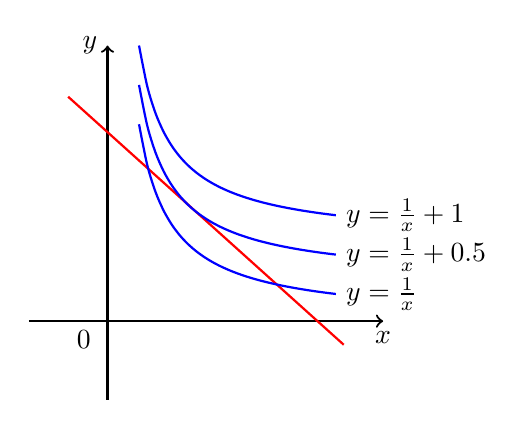
\begin{tikzpicture}[scale=1]
	
	\draw [thick, ->] (-1,0) -- (3.5, 0) node [anchor = north] {$x$};
	\draw [thick, ->] (0,-1) -- (0,3.5) node [anchor=east] {$y$};
	
	\node [below] at (-0.3,0) {$0$};
	\draw[domain=-0.5:3, smooth, thick, , variable = \x, red, text=black] plot ({\x}, {-0.9*\x+2.4});
	\draw[domain=0.4:2.9, smooth, thick, , variable = \x, blue, text=black] plot ({\x}, {1/(\x)}) node[right]{$y=\frac{1}{x}$};
	\draw[domain=0.4:2.9, smooth, thick, , variable = \x, blue, text=black] plot ({\x}, {1/(\x)+1}) node[right]{$y=\frac{1}{x}+1$};
	\draw[domain=0.4:2.9, smooth, thick, , variable = \x, blue,text=black] plot ({\x}, {1/(\x)+0.5}) node[right]{$y=\frac{1}{x}+0.5$};
	\end{tikzpicture}
	\end{center}
		
	Put $k=y - \frac{1}{x}$.
	
	$k=y-\frac{1}{x}$ has the form of graph as illustrated as blue graphs. The graph should satisfy the following conditions: it should be on the region--some point on the graph should also be on the region--and it should make $k$ maximum. Combining these two conditions, we can conclude that the graph should be as high as possible about $y$-axis, still meeting the region. Since $y = \frac{1}{x}+k$ has derivative $y' = -\frac{1}{x^2}$ on $(0,\infty)$, we can conclude that there exists some $(x,y)$ such that $y' = -0.9$. That is, there exists $k$ such that $y = \frac{1}{x} + k$ tangent to $y=-0.9x +2.4$. By calculations, two graphs meet tangentially at the point $(\frac{\sqrt{10}}{3}, -\frac{3\sqrt{10}}{10}+2.4)$. By putting this value into $y = \frac{1}{x} +k$, we get the maximum $k=-\frac{3}{5}\sqrt{10}+2.4$
	
	We will see specific implementation of ILP in Section \ref{section-ILP imp}
	
	\section{Rules of the game Rummikub}\label{section-rules}
	
	%이걸 설명해야하나 아니면 이걸 보라고 하면 되겠지 그냥?
	
	There are total 106 tiles--2 sets of tiles numbered 1 to 13 in four colors: black, red, blue, orange; 2 Jokers. There are 4 racks that the players can put their tiles on, hence 2 to 4 players can join the game.
	meld
	A set is ~
	Each players has a turn and when it is one's turn, that player give out sets or 
	A group is a set of either three or four tiles of the same number in different colors.
	A run is a set of three or more consecutive numbers, all in the same color.
	
	Scoring system

	
	
	\section{ILP on Rummikub}\label{section-ILP imp}
	
	There are two goals of this programming:\\
	(1) The major goal is to maximize the number of value of the tiles that can be placed onto the table.\\
	(2) The minor goal is to minimize the movement of the existing sets on the table.\\
	It seems like this programming is a greedy algorithm if we only look over the major goal. However, in order to consider real practice, 
	
	
	
	The ILP model is implemented in AIMMS (Advanced Integrated Multi-Dimensional Modelling Software) on a Pentium %3 로마자로
	
	

	%anyone can do until now



	\section{ILP on My First Rummikub}\label{section-ILP MFR}

	%이걸 직접 해보기


	\section{Implementation}\label{section-imp}
	
	%아니면 어떤 걸 써야할 것 같은지에 대새 쓰고 implementation 은 기말 과제로!
	There are ~ goals of this programming:\\
	(1) Maximize the number of value of the tiles that can be placed onto the table.\\
	(2) Maximize 
	% 1이랑 13 같이 끼워맞추기 어려운--이걸 수학적으로? 숫자는 먼저 낸다. 큰 수는 먼저 낸다 (점수에 반영)
	
	%scoring 에 영향을 주기 위해서는 어떻게 하면 좋을까. 어차피 다 내는 걸 목표로 해야할 텐데...
	
	
	
	
	
	\bibliographystyle{alpha}
	\bibliography{references} % see references.bib for bibliography management
	
\end{document}
 